\documentclass[notumble,combine]{leaflet}
\usepackage[dvipsnames,usenames]{color}
\usepackage{graphicx}
\usepackage{alltt}
\usepackage{url}
\usepackage{ascmac}
\usepackage{comment}
\usepackage{here}
\usepackage{wrapfig}

\makeatletter
% from leaflet.cls
\renewcommand\section{\@startsection{section}{1}{\z@}%
  {-3.5ex \@plus -.75ex}%
  {1ex} %{1.5ex}%
  {\normalfont\large\sectfont\color{NavyBlue}}}
\renewcommand\subsection{\@startsection{subsection}{2}{\z@}%
  {-2.5ex plus -.5ex}%
  {1\p@} %{1ex}%
  {\normalfont\normalsize\sectfont\color{BrickRed}}}
\makeatother

\graphicspath{{figures/}} 

\title{
	\vfill
	\includegraphics[width=\textwidth]{kbug-logo}
	\vfill
	\resizebox{\linewidth}{!}{\bf 関西*BSDユーザ会}%
	\\[\baselineskip]
        \resizebox{\linewidth}{!}{{\bf \url{http://www.kbug.gr.jp/}}}
	\vfill
        \parbox[c]{3cm}{\resizebox{3cm}{!}{\textcolor{red}{\bf{@}}}}
	
\includegraphics[width=\textwidth]{banner2009}
        \resizebox{\linewidth}{!}{{\bf \url{http://k-of.jp/2009/}}}\\
        \resizebox{\linewidth}{!}{2009年11月6日(金),7日(土)}
}

\date{}

\begin{document}
\maketitle
\thispagestyle{empty}
\pagebreak{}
\section{関西*BSDユーザ会ってなに?}
関西 *BSD ユーザ会 (Kansai *BSD Users Group; K*BUG)とは、
BSD系OSのユーザ同士の情報交換のための{\em 場}で、1999年に作
成されました。

年に数度(大体2ヶ月に1度程度)の勉強会や宴会を行っています。

\subsection{K*BSDの基本理念}
K*BUGの基本理念は以下のようになっています
(\url{http://www.kbug.gr.jp/charter.html}より)。

\fbox{\begin{minipage}{\textwidth}
\begin{itemize}
\item 場の提供を目的とする
\item 人のケツは叩くが足は引っ張らない
\item 来るものは拒まず、猿ものは追わず
\item だれでも役員になれる。誰でも役員は止められる
\end{itemize}
\end{minipage}}
\begin{wrapfigure}[8]{r}{3cm}
\begin{center}
 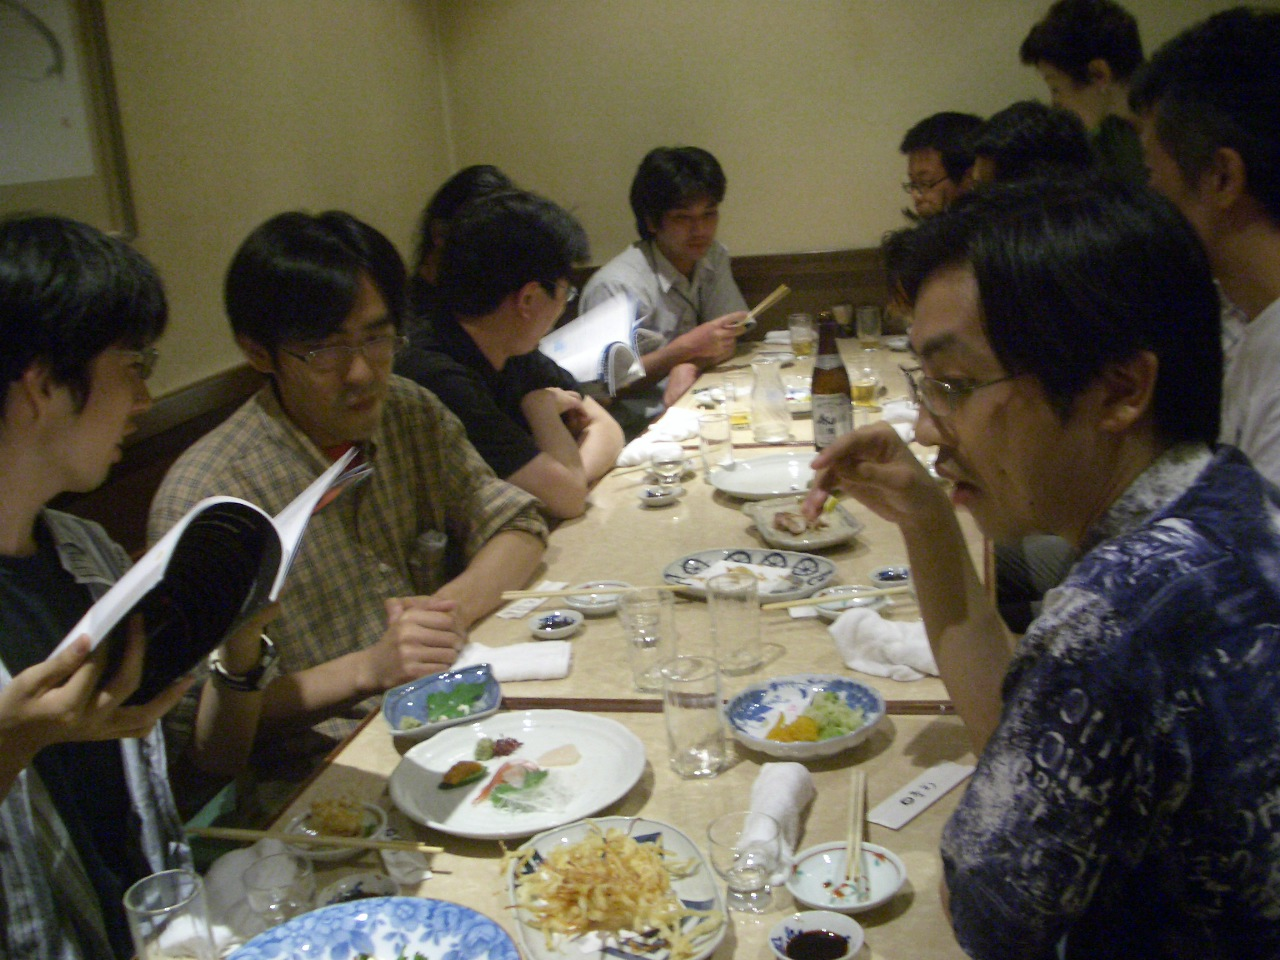
\includegraphics[width=3cm]{CIMG2521}\\
 飲み会は大切
\end{center}
\end{wrapfigure}

少し難しく感じるかもしれないですが、\textcolor{red}{BSDへの愛と情熱}があれば、
あなたが\textcolor{blue}{やりたいと思うことができる場}がK*BUGなのです。

また、メンバーは色々な技術に詳しいですし、技術に関する話も大好きなので、
あなたの疑問などもぶつけてみてください。

\section{最近の活動}
KOF2008からの最近の活動とその内容は以下のとおりです。

もし、興味のあるテーマがあるようでしたら、是非一度遊びにきてください。

\subsection{2009年9月12日(土)@大阪}

\subsection{2009年7月25日(土)@京都}
\begin{itemize}
\item 家計簿をつけよう
\item 「BPG4で遊ぼう」\footnote{\url{http://genta.teeda.jp/materials/20090725_01_KBUG_Genta_IHA.pdf}}
\item 番外:酔っぱらいのための割り勘計算
\end{itemize}

\subsection{2009年7月10日(金),11日(土) OSC2009 Kansai@京都}

OSC2009 Kansai\footnote{\url{http://www.ospn.jp/osc2009-kansai/}}で、ブースを設置しました。
JNUGさんとはおとなりです。

\begin{itemize}
\item NetBSDなひととき
\item 展示
\item ブース企画
\begin{itemize}
\item bcbench \footnote{\url{http://www.yagoto-urayama.jp/~oshimaya/nbug/etc/bench/bcbench.html}}チキンレース
\item 夏の京都恒例:電力測定
\end{itemize}
\end{itemize}

\subsection{2009年5月16日(土)@神戸}
\begin{itemize}
\item モダンDNS入門
\item Typolight2.7の紹介
\item llvm/clangでFreeBSD
\item ベーグルボードとInterface付属ボードもってきたよ回覧
\item モバイルギアでNetBSD
\end{itemize}

\subsection{2009年3月28日(土)@N:KM京都}
むとうがSqueak-jaと共同でブースを出しました\footnote{\url{http://qml.610t.org/squeak/mutoh_20090321.html}}。
\begin{itemize}
\item Design Wave Magazine + Squeak + FreeBSD = Drive a Car!!
\item PicoBoard + Scratch + FreeBSD = まわる猫
\item Squeak+Gainerの世界
\item 歴代世界聴診器集合
\item PDA de Squeak
\end{itemize}

\subsection{2009年3月7日(土)@大阪}

\subsection{2009年1月24日(土)@京都}
\begin{itemize}
\item RemotePad for iPhoneの開発について
\item FreeBSDのsetfibについて
\item FreeBSDでのgainerの利用について
\item Gainer miniとCでの使い方
\item uipaq0ネタ
\item NetBSDのtime\_t 64bit化について
\item TigerのFSEvents APIについて
\end{itemize}

\subsection{2008年12月6日(土)総会@大阪}

\subsection{2008年11月7日(金), 8日(土)KOF2008@大阪}
\begin{wrapfigure}{r}{3cm}
\begin{center}
 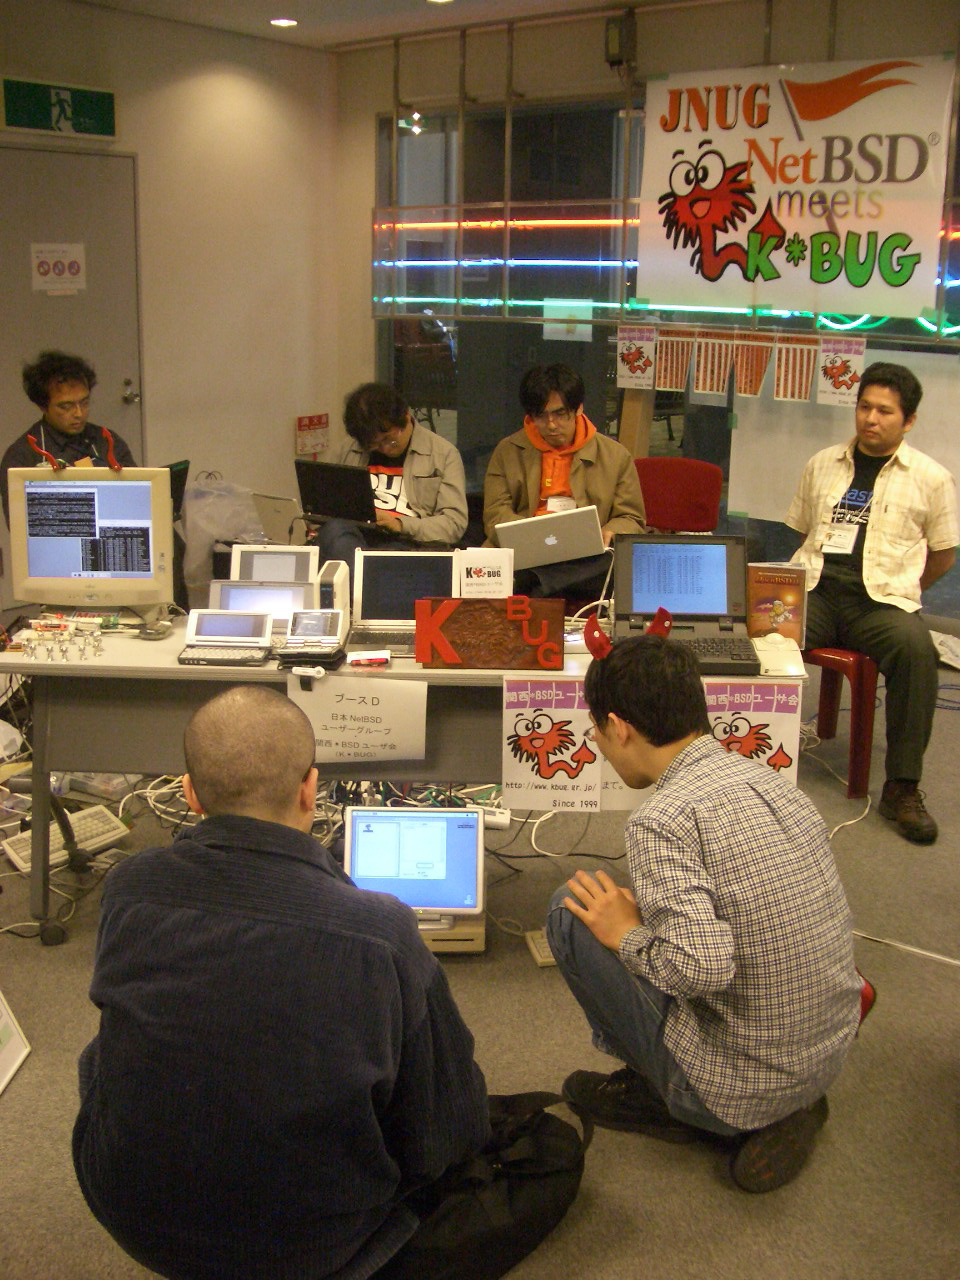
\includegraphics[width=3cm]{CIMG3131}%\\
\end{center}
\end{wrapfigure}

KOF2008\footnote{\url{http://www.ospn.jp/osc2008-kansai/}}で、JNUGさんと共同ブースを設置しました。

\begin{itemize}
\item NetBSDなひととき
\item 展示
\begin{itemize}
\item {\em 恒例、色々なオールドマシンがBSDで動く!!}
\item USL-5P/NetBSDによるLED照明システム
\item NetBSD uvideoで遊ぼう
\item Squeak+Gainer/FreeBSD
\item 趣味の木彫看板
\end{itemize}
\end{itemize}

\subsection{その他}
以下のようなURLで、メンバーの発表が紹介されていますので、活動内容を知るための参考にしてください。
\begin{itemize}
 \item \url{http://hp.vector.co.jp/authors/VA012337/misc/presentation.html}
 \item \url{http://qml.610t.org/FreeBSD/BUG.html}
\end{itemize}

\pagebreak{}
\section{K*BUG@KOF2009 Kansai}
\subsection{展示}
\begin{itemize}
 \item 魅惑のえびじゅんコレクション「旅するトランク」
 \item 僕らの工作: 木彫やぬいぐるみも!!
 \item \textcolor{red}{\Large 他にもたくさんの○○BSDが…}
\end{itemize}

\section{BSDに関する情報}
\subsection{リンク集}
\begin{itemize}
\item JNUG(Japan NetBSD Users Group)\\
  今回もブースをご一緒させてもらいました\\
  \url{http://www.jp.netbsd.org/}
\item FreeBSD友の会  \url{http://www.jp.freebsd.org/}
\item OpenBSD本家  \url{http://www.openbsd.org/ja/}
\item Dragonfly BSD \url{http://dragonflybsd.org/}
\item 名古屋*BSDユーザグループ \url{http://www.nagoya.bug.gr.jp/}
\item 四国*BSDユーザ会 \url{http://flathill.gr.jp/sbug/}
\end{itemize}

\pagebreak{}
\section{これからの関連イベント(予定)}
詳細は、Webページをご確認ください。

\begin{itemize}
\item \textcolor{red}{\Large 来週!!}2009年11月14日(土) 第6回研究会@京都
\item 2009年12月5日(土) 定期総会+第7回研究会+忘年会@大阪
\item 2010年 3月11日(木)-14(日) AsiaBSDCon 2010 \footnote{\url{http://2010.asiabsdcon.org/}}
\end{itemize}

\section{「BSDなひととき」}
以下のように「BSDなひととき」を行いますので、ご参加ください。

\begin{itemize}
\item 日時: 2009/11/7 16:00-16:50 (50 min)
\item 会場: 9Fセミナー2
\item 講師: 蛯原 純 (The NetBSD Project/株式会社創夢)
\item 主催:日本NetBSDユーザーグループ
\item \url{http://k-of.jp/2009/list_seminar.html#34}
\end{itemize}

BSD系UNIXを取り巻く環境と、将来の展望について議論し、BSDコミュニティ間の情報交換を行なうBOFセッションです。
BSD系UNIX全般を対象とした幅広いテーマで議論します。 

\begin{comment}
BSD系UNIXを取り巻く環境と、将来の展望について議論し、 BSDコミュニティ間の情報交換を行なうBOFセッションです。
4.4BSDの流れをくむFreeBSD/NetBSD/OpenBSDなど、 BSD系UNIXのユーザグループ合同で、BSD系UNIX全般を対象とした幅広いテーマで議論します。
\end{comment}

\vfill

\begin{minipage}{\textwidth}
\begin{boxnote}

\section{kbug-usersメーリングリスト}
K*BUGでは、K*BUGメンバーの情報交換や、イベントなどの情報伝達用に
kbug-usersメーリングリストを用意しています。

K*BUGメンバーは、基本的にはこのメーリングリストを読んでいることが期待
されます。

購読は以下のURLをご参照ください。
\begin{itemize}
 \item \url{http://www.kbug.gr.jp/maillist.html}
\end{itemize}
\end{boxnote}
\end{minipage}

\end{document}  
